\documentclass[a4paper,12pt,titlepage]{article}

\usepackage{listings}
\usepackage{amsmath}
\usepackage{amssymb}
\usepackage{amsthm}
\usepackage{graphicx}
\usepackage{hyperref}
\usepackage{parskip}
\usepackage{pdfpages}

\setlength{\parindent}{15pt}
\hypersetup{colorlinks=true,linkcolor=green}

\begin{document}

\title{Network Security Class \\ Lab Session 3}
\author{Stefano Zanella - 621796}
\date{July 2013}

\maketitle

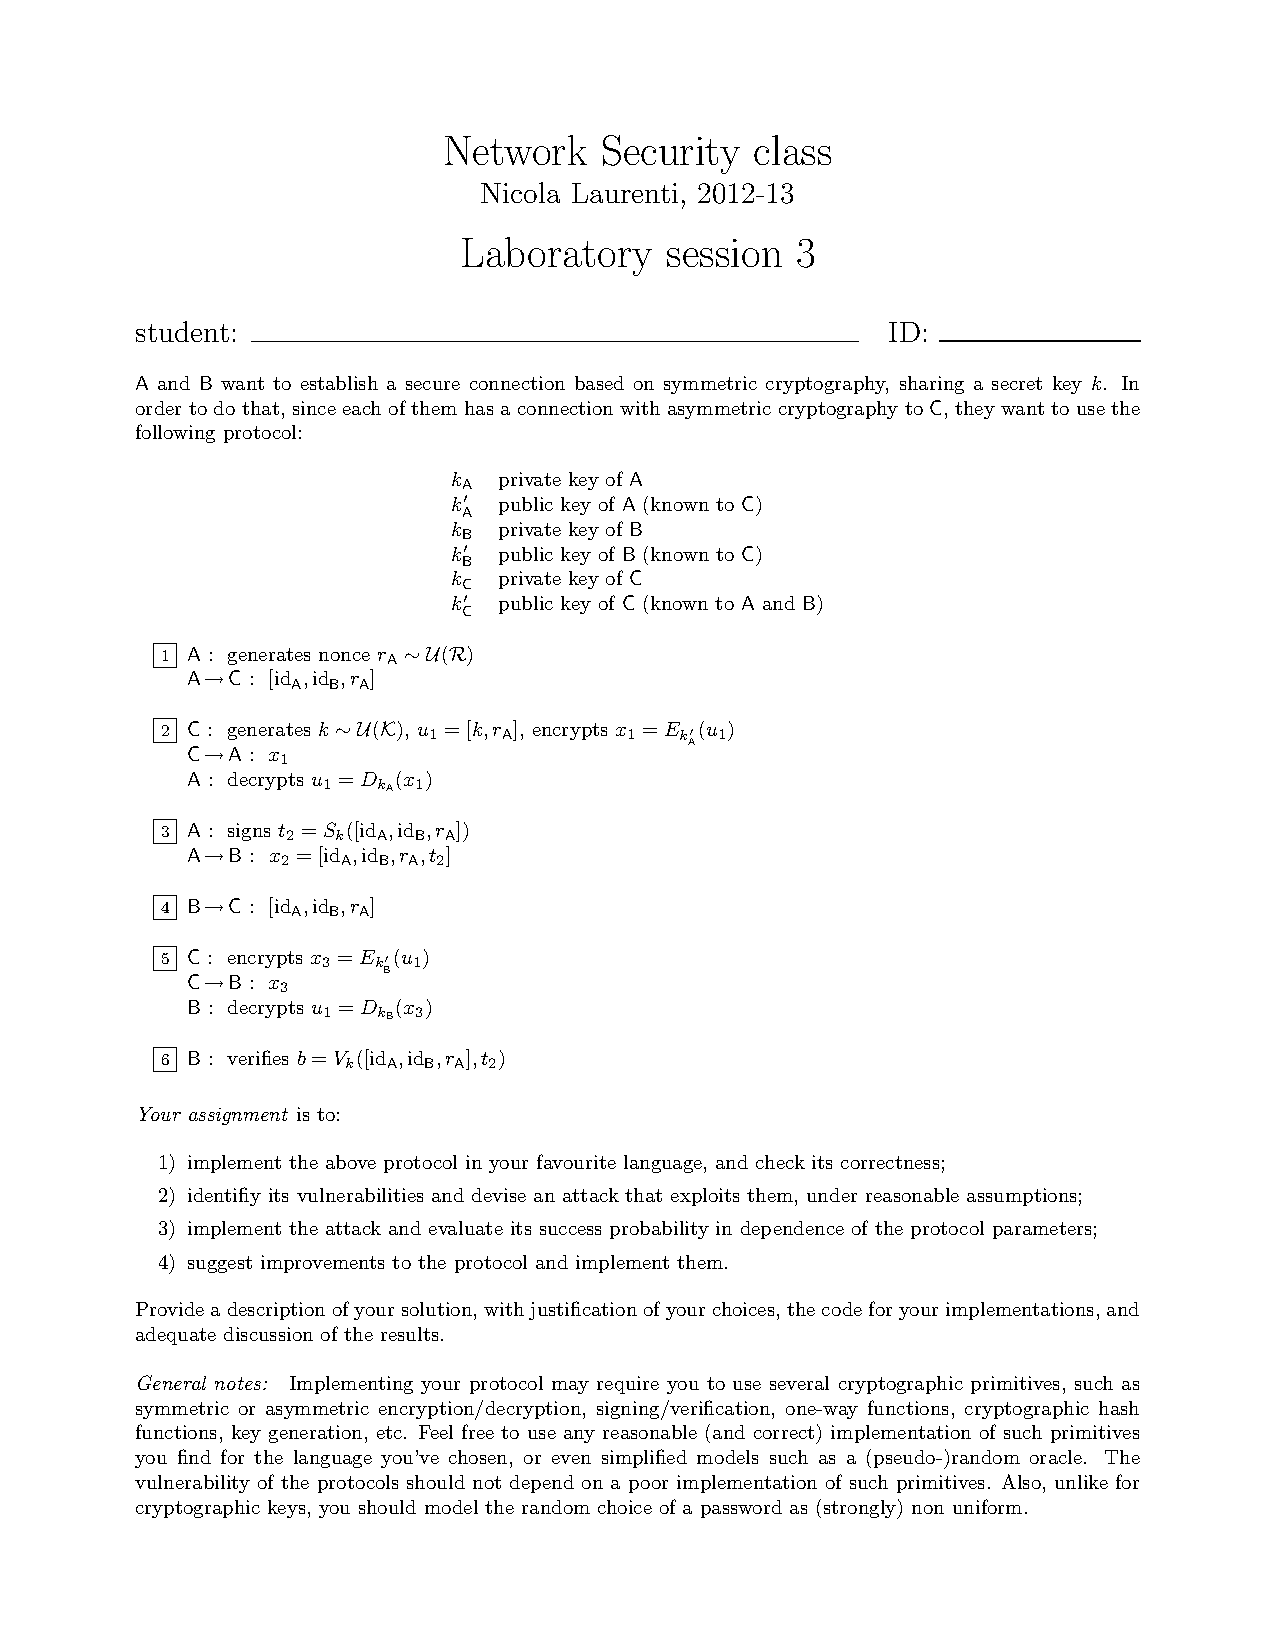
\includepdf[pages={1}]{lab_3_assignment.pdf}

\section{Implementation Details}
Here are the choices made where requested by the assignment or when no further
specification given:

\begin{itemize}
	\item The assignment has been implemented in \textbf{Ruby} (version \textbf{2.0.0-p195})
	\item To simplify the resulting codebase hosts have been modeled as classes, and
        communications over the network channel have been modeled with a \texttt{Channel}
        class that acts like a simple shared message storage. This allows to easily
        simulate message exchanging and eavesdropping.
	\item For the same reason, and to make the source code more readable, data
        concatenation has been modeled with hash maps. This in fact replaces
        specifying data chuncks' lengths in the protocol with specifying the keys at
        which data chuncks are accessible.
	\item Cryptographic primitives (ciphers, RNGs, etc.) are provided by Ruby's wrapper
        around the \textbf{OpenSSL} library and core language facilites. In detail:

    \begin{itemize}
      \item RNG is provided by the built-in \texttt{Random} class
            (\href{http://ruby-doc.org/core-2.0/Random.html}{documentation}), a PRNG based
            on a \emph{Mersenne twister}.
      \item asymmetric public key algorithm is RSA (Ruby
            \href{http://www.ruby-doc.org/stdlib-2.0/libdoc/openssl/rdoc/OpenSSL/PKey/RSA.html}{documentation}),
            with \textbf{2048 bits} key length.
      \item symmetric key cipher is \textbf{AES 256}, used when simulating communications
            between nodes.
      \item message authentication/integrity protection is provided by class \texttt{OpenSSL::HMAC}, which accepts
            an available digest algorithm as a parameter. Selected cryptographic hash
            function for message authentication is \textbf{SHA512}, provided by class
            \texttt{OpenSSL::Digest::SHA512}
            (\href{http://www.ruby-doc.org/stdlib-2.0/libdoc/openssl/rdoc/OpenSSL/Digest.html}{documentation}).
    \end{itemize}

	\item Since OpenSSL RSA works on strings, all hashes used for communication needed
  to be serialized before encryption. Ruby's built-in standard for
  serialization/deserialization is \textbf{YAML}
  (\href{http://www.ruby-doc.org/stdlib-2.0/libdoc/yaml/rdoc/YAML.html}{documentation}),
  which use is made transparent by encapsulation into class \texttt{NetSec::Node}.
\end{itemize}

\section{Protocol Implementation}
Given protocol is implemented in \texttt{NetSec::KeyExchange\#start!} method. \\
Correctness is proven at the end by printing keys hold by \textbf{A} and \textbf{B},
which are obviously the same in case the protocol works correctly.

To run the exchange, just type at the prompt, from inside the source folder:

\begin{lstlisting}[language=bash]
bin/key_agreement
\end{lstlisting}

The output should be something similar to:

\begin{lstlisting}[language=bash]
A has key: ["a2b85f3a7164c411d8ea5eb66affa741472eb59be787
                                   c3b3ea63b7816c868d39"]
B has key: ["a2b85f3a7164c411d8ea5eb66affa741472eb59be787
                                   c3b3ea63b7816c868d39"]
\end{lstlisting}

\section{Possible Flaws and Related Attacks}
\subsection*{C Node Spoofing}
While \textbf{C} makes use of asymmetric cryptography to exchange the key with
\textbf{A} and \textbf{B}, these last two does not the same when communicating with
\textbf{C}. This easily allows an attacker to spoof \textbf{C}'s identity (for example,
by DoSing it and routing requests to itself); once the attacker can
successfully impersonate \textbf{C} it has just to save the list of generated keys
and start eavesdropping from the communication channel. This way it can do
whatever it wants (from simply logging exchanged information to manipulation of
exchanged data), given no other security mechanisms are in place for a given
session (e.g. for message integrity).

\section{Attacks Implementation and Analysis}
\subsection*{C Node Spoofing}
To simulate spoofing of node C, a \texttt{NetSec::SpoofedC} subclass has been
introduced. Basically it acts the same way as its parent class, plus it
eavesdrop on the channel upon initialization and then saves the generated key
to decrypt eavesdropped messages.

Spoofing simulation can be run from the prompt by invoking:

\begin{lstlisting}[language=bash]
bin/spoofing_attack
\end{lstlisting}

which outputs something along the lines of:

\begin{lstlisting}[language=bash]
A has key: ["c26c3f32631b6eb395d90a63f835baccbdbc244cd400
                                   a15312bbfea15bffa93b"]
B has key: ["c26c3f32631b6eb395d90a63f835baccbdbc244cd400
                                   a15312bbfea15bffa93b"]
Spoofed C has key: ["c26c3f32631b6eb395d90a63f835baccbdbc
                           244cd400a15312bbfea15bffa93b"]
B received: My credit card number is 1234567890123456
The attacker eavesdropped: My credit card number is 
                                   1234567890123456
\end{lstlisting}

\section{Possible Improvements}
\subsection*{C Node Spoofing}
A simple solution to the problem of spoofing \textbf{C} identity would be to make
use of \textbf{C} asymmetric keys during key agreement. \\
In particular, in steps \textbf{1} and \textbf{4}, \textbf{A} and \textbf{B} could encrypt the
message $[id_A, id_B, r_A$] using \textbf{C}'s public key
$k_C'$. On the other side, \textbf{C} would then decrypt received messages
using its private key $k_C$. With this simple improvement, the only
way for an attacker to perform the same spoofing attack would be to steal
\textbf{C}'s private key, which is supposed to be an event with low probability of
success given the assumptions on which  asymmetric cryptography is based.

This solution is implemented in classes \texttt{AntispoofingA}, \texttt{AntispoofingB} and
\texttt{AntispoofingC}. The correctness of the implementation can be seen by launching
from the prompt:

\begin{lstlisting}[language=bash]
bin/antispoofing_agreement
\end{lstlisting}

To simulate the attack against this improved version, class
\texttt{SpoofedAntispoofingC} has been created. By launching

\begin{lstlisting}[language=bash]
bin/antispoofing_attack
\end{lstlisting}

it can be seen how the whole process generates an error when the malicious
\textbf{C} tries to decrypt the message from \textbf{A}'s step 1 without having the
correct private key.
\end{document}
